\chapter{Použitie viacerých template štruktúr pri predikcií}

Ako druhé opatrenie, na zlepšenie rýchlosti a presnosti predikovania nekonzerovvaných úsekov sme navrhli  použiť viacero template štruktúr na predikciu jednej target štruktúry. Očakávali sme pritom, že sa nám podarí zmenšiť počet a dĺžku nekonzervovaných úsekov v predikovanej štruktúre a tým výrazne zjednosušiť ich predikciu algoritmom FARFAR.

\section{Výber sekundárnych template štruktúr}
Hlavnou myšlienkou algoritmu je použiť viacero template štruktúr pre predikciu jednej target štruktúry. Tým môžeme dosiahnuť väčšiu percentuálnu mieru konzervovaných úsekov v štruktúre, čo by malo zjednodušiť následnu predikciu nekonzervovaných úsekov.


\indent  Existuje viacero spôsobov, ako je možné použiť na predikciu viacero template štruktúr. My sme sa aj vzhľadom na jednoduchšiu implementáciu do už existujúceho algoritmu rozhodli postupovať tak, že používame jednu template štruktúru ako primárnu (hlavnú) a ďalšie template štruktúry, ako sekundárne (vedľajšie), ktoré sú použité na vyplnenie dlhých nekonzervovaných úsekov (to sú tie, ktoré v pôvodnom algoritme vyčleňujeme do samostatných predikcií). Alternatívny prístup by mohol byť rozdeliť si target sekvenciu na regióny a pre predikciu každého regiónu použiť inú template štruktúru.   


\indent Potencionálnych spôsobov ako nájsť vhodnú sekundárne štruktúry existuje viac: 
\begin{enumerate}
\item Globálne zarovnanie potenciálnych sekundárnych temeplate molekúl s target molekulou. 
\item Lokálne zarovnanie potenciálnych sekundárnych tmeplate molekúl s target molekulou. 
\item Semiglobálne zarovnanie potenciálnych sekundárnych temeplate molekúl s target molekulou. 
\item Najprv zarovnať heuristickým algoritmom (BLAST, FASTA) a následne z takto vybranej skupiny najlepších štruktúr vybrať tú najvhodnejšiu za pomoci jedného z troch hore uvedených spôsobov.
\end{enumerate}


\indent My sme najprv skúšali prvý a najjednoduchší postup a to globálne zarovnávať potencionálne sekundárne molekuly na target molekulu pričom v zarovnaniach hľadáme sekundárnu štruktúru, ktorá by dobre vyplnila nekonzervované úseky (teda by ich pokryla aspoň na 60\%, ktoré sme na základe doterajšieho testovania určili ako dolnú hranicu pokrytia v zarovnaní). Pri globálnom zarovnaní sme však nenachádzali vhodné sekundárne štruktúry, ktoré by pokrývali nekonzervované úseky s aspoň 60\%. Je to dané tým, že okrem toho, že v sekundárnej template štruktúre sa musí nachádzať vhodný konzervovaný úsek musí byť aj na správnom mieste v štruktúre tak, aby bol globálne zarovnaný na miesto nekonzervovaného úseku v target štruktúre. Tento prístup sme nakoniec označili za nepoužiteľný.


\indent Lokálne zarovnanie hľadá zarovnanie s najlepším skóre dvoch podúsekov z target aj template sekvencie. To znamená, že dĺžka zarovnaných úsekov je určená najvyšším skóre zarovnania oboch sekvencií (ak by bol do zarovnania pridaný alebo odobratý ľubovolný nukleotid z target alebo template sekvencie skóre zarovnania by sa zhoršilo). Vzhľadom na to, že my potrebujeme zarovnať celý nekonzervovaný úsek target sekvencie na ľubovoľný úsek template sevencie bolo by lokálne zarovnanie ťažko použiteľné.


\indent Semiglobálne zarovnanie je kombinácia globálneho a lokálneho zarovnania. Funguje tak, že kratšiu štruktúru zarovná na časť dlhšej štruktúry a nezarovnané úseky pred a po kratšej štruktúre sa do výsledného skóre zarovnania nezapočítavajú. Teda z globálnym zarovnaním má spoločné to, že kratšia sekvencia je zarovnaná celá na časť dlhšej. Z lokálnym zarovnaním má spoločné to, že pridaním alebo odobratím ďalšieho nukleotidu z dlhšej štruktúry do zarovnania by sme výsledné skóre len zhoršili. V našom algoritme ho budeme používať na vyľadanie optimálnych sekundárnych template molekúl. Postupovať tak, že vyberieme nekonzervovaný úsek z target sekvencie a postupne ho budeme zarovnávať na rôzne potencionálne template sekvencie. Buď môžeme prejsť všetky dostupné sekvencie pre každý nekonzervovaný úsek a vybrať najlepšiu, alebo vyberieme prvú ktorá splní nejaké nami zadané požiadavky. Nevýhoda prechádzania všetkých sekvencií je vysoká časová náročnosť, pretože algoritmus zarovnania má kvadratickú časovú náročnosť O(mn), kde m a n sú dĺžky zarovnávaných molekúl. Teda asymptotoicky bude náročnosť predikcie jednej štruktúry O(snm), kde n a m sú dĺžky štruktúr a s je počet štruktúr v databáze. 


\indent Semiglobálne zarovnanie získavame rovnakým nástrojom ako globálne, teda pomocou programu Emboss.Needle \cite{Emboss}. Z výsledného zarovnania nás nezaujíma skóre zarovnania, ale percentuálny pomer správne zarovnaných nukleotidov oproti nesprávne zarovnaným nukleotidom, prípadne medzerám v  zarovnaní (bez medzery na začiatku a na konci), čo označujeme ako podobnosť, alebo tiež similarity. Emboss ale do výstupného súboru zarovnania uvádza len globálnu podobnosť v kombinácií so semiglobálnym skóre \ref{obr06:emboss}. To pre nás znamenalo, že sme muslei napísať parser založený na regulárnych výrazoch, ktorý vyselektuje zo zarovnania len zarovnanú časť a určí podobnosť oboch štruktúr.
\begin{figure}%[p]\centering
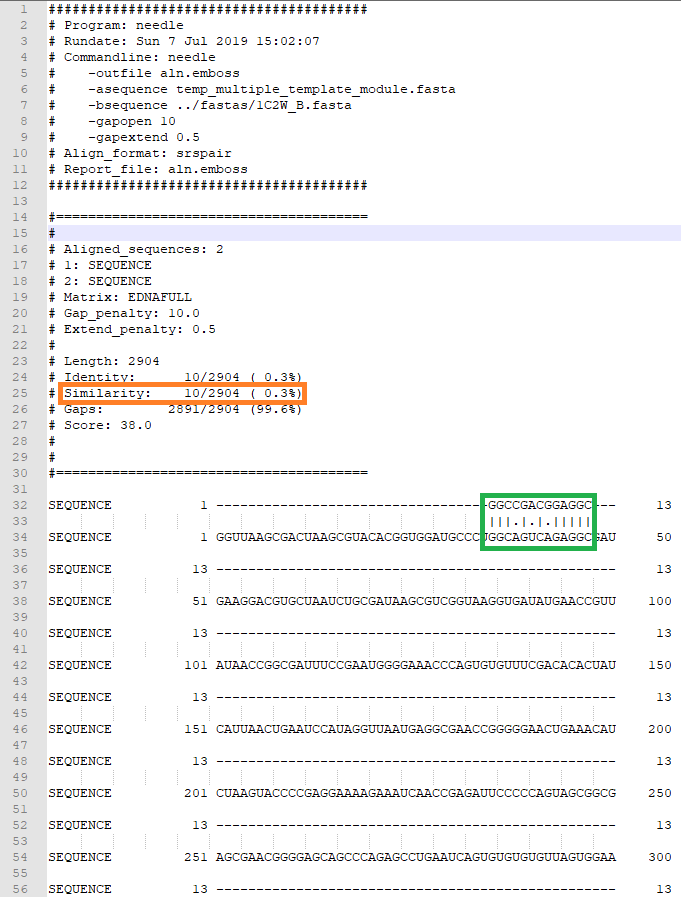
\includegraphics[width=\textwidth]{../img/emboss}
\caption{Príklad semiglobálneho zarovnania nekonzervovaného rozšíreného úseku dlhého 13 nukleotidov na sekvenciu 1C2W\_B dlhú 2904 nukleotidov. Zeleným obdĺžnikom je ohraničené zarovnanie, ktorého podobnosť nás zaujíma a oranžovým obdĺžnikom je označená hodnota globálnej podobnosti vypočítanej programom Emboss.}
\label{obr06:emboss}
\end{figure}


\indent Zvýšená časová náročnosť by sa dala riešiť použitím algoritmov FASTA, ktoré používajú heuristické metódy na vyhľadanie najpodobnejších sekvencií. V našom prípade, kedy máme približne 1500 sekvencií na porovnanie, trvá presný semiglobálny alignment niekoľo minút a vzhľadom na to, že neskoršia de novo predikcia trvá oveľa dlhšie, rozhodli sme sa tento problém neriešiť.


\section{Algoritmus}
\indent Kroky algoritmu používajúceho viacero sekundárnych template štruktúr:
\begin{enumerate}
\item Nájdeme dlhé nekonzervované úseky.
\item Otagujeme a vyfiltrujeme potenciálne template štruktúry sekvenčným prechodom všetkých štruktúr, uložíme  ich do poľa.
\item For each nekonzervovaný úsek:
\begin{enumerate}
\item Upravíme nekonzervovaný úsek na rozšírený nekonzervovaný úsek (o úseky, ktorými budeme spájať s primárnou target štruktúrou).
\item Pomocou semiglobálneho zarovnania nájdeme v indexovaných štruktúrach vhodnú sekundárnu štruktúru pre nekonzervovaný úsek.
\item Namapujeme vybraný fragment sekundárnej target štruktúry na príslušné miesto v template štruktúre (prečíslovanie nukleotidov v sekundárnej template štruktúre).
\item Vykonáme jeden z následujúcich dvoch krokov, podľa verzie algoritmu:
\begin{enumerate}
\item Dáme do superpozície štruktúru tvorenú konzervovanými úsekmi z primárnej template štruktúry a fragment zo sekundárnej štruktúry.
\item Uložíme fragment sekundárnej template štruktúry do separátneho súboru.
\end{enumerate}
\end{enumerate}
\end{enumerate}


\indent Hlavná logika je naimplementovaná v skriptoch \url{Predictor/scripts/multiple\_templates\_modul.py} a \url{Predictor/scripts/superposition.py}. Druhý z menovaných skriptov bol pôvodne inšpirovaný skriptom od Anders S. Christensen-a dostupného na \url{https://gist.github.com/andersx/6354971}, a výrazne upravený.  


\indent V prvom kroku sekvenčne prejdeme target štruktúru skladajúcu sa zatiaľ len z konzervovaných úsekov primárnej template štruktúry a vyhľadáme nekonzervované úseky dlhšie ako určitá hranica daná parametrom (momentálne nastavené na 7 nukleotirdov).


\indent V druhom kroku si predpripravíme možné template štruktúry tak, že odstránime tie, ktoré obsahujú moc veľa neplatných nukleotidov (znaky iné ako A,C,G,U), ale hlavne si uložíme dĺžku každej sekvencie a v nasledujúcom kroku budeme na seba zarovnávať len dosť dlhé sekvencie vzhľadom k nekonzervovanému úseku (minimálne 0,8 násobok dĺžky úseku). Dôvody sú vyhnutie sa problémovým dátam a ušetrenie času pri zarovnávaní hlavne dlhších nekonzervovvaných úsekov. Tu by bolo možné si takto sekvencie otagovať mimo algoritmu predikcie, čo by ale bolo treba prepočítavať pri zmene v databázi, a keďže celý tento proces trvá pár desiatok sekúnd rozhodli sme sa robiť to vždy odznova počas predikcie.


\indent V ďalších krokoch iterujeme cez všetky vybrané nekonzervované úseky algoritmu a pre každý aplikujeme rovnaké kroky. Najprv si nekonzervovvaný úsek rozšírime. To znamená, že k nemu pridáme z oboch strán určitý počet nukleotidov (my používame parameter 5). Keďže pracujeme s nekonzervovvaným úsekom musí existovať na každej strane minimálne 1 nukleotid, ktorý tento úsek ohraničuje (s výnimkou začiatku a konca sekvencie). Za pomoci týchto rozširujúcich nukleotidov sme schopní superpozíciovať (správne umiestniť) v nasledujúcich krokoch vybraný fragment sekundárnej template štruktúry do primárnej template štruktúry.


\indent V tomto kroku postupne zarovnávame rošírený nekonzervovaný úsek s vyhovujúcimi predpripravenými štruktúrami z druhého kroku. V prípade, že zarovnanie splňuje určené podmienky, vyberieme príslušnu štruktúru za sekundárny template  pre spracovávaný nekonzervovaný úsek a v prehľadávaní ďalej nepokračujeme. Podmienky pre výber používame nasledujúce: podobnosť zarovnania minimálne 70\% a maximálne 95\%. Maximálnu podobnosť volíme preto, aby sme ako template nepoužili štruktúru skoro úplne zhodnú s target štruktúrou. To by síce bolo žiaduce pri naozajstnej predikcii kedy chcem dostať čo najlepší výsledok, ale nežiadúce pre testovanie funkčnosti predikcie, kedy by nám to zvyšok predikcie výrazne zjednodušilo. Pri predikcií neznámej štruktúry tiež typicky nepoznáme žiadnu veľmi podobnú štruktúru neznámej štruktúre, inak by sme ju použili ako primárny template. 


\indent V ďalšom kroku musíme namapovať nukleotidy zo sekundárnej template štruktúry do nekonzervovaného úseku primárnej template štruktúry (ktorá je už namapovaná na target sekvenciu) podľa zarovnania. To znamená pre každý použitý nukleoti zistiť, na aký nukleotid bol namapovaný a zmeniť jeho index v pdb súbore. Okrem toho musíme zmeniť aj chain ID v prípade, že sa nezhodujú chain ids primárnej a sekundárnej template štruktúry.


\indent V poslednom kroku sme skúšali dva rôzne spôsoby. 
Prvý bol superpoziciovať nukleotidy, ktorými sme rozšírili z oboch strán nekonzervovaný úsek na odpovedajúce nukleotidy v primárnej template štruktúre. Inak povedané to znamená vhodným spôsobom rotovať a posúvať sekundárnu template štruktúru ako celok tak, aby sme minimalizovali RMSD nukleotidov, ktoré majú v oboch štruktúrach rovnaké indexy. Na toto sme použili Superimposer implementovaný v knižnici BioPython. Po vhodnej rotácií a translácií sekundárnej template štruktúry z nej odstránime pridané rozširujúce úseky a nukleotidy čiastočne pokrývajúce nekonzervovaný úsek skopírujeme do primárnej templae štruktúry. Takýmto spôsobom v ideálnom prípade vyplníme jeden dlhý nekonzervovaný úsek v primárnej template štruktúre, fragmentom štruktúry zo sekundárnej target štruktúry. Vo výsledku by sme pri použití prvého prístupu mali template štruktúru, ktorá má dodatočne doplnené dlhé nekonzervované úseky vhodnými fragmentmi ostatných štruktúr.
Druhý prístup je jednoduchší a pozostáva len z uloženia správne namapovaných fragmentov sekundárnej štruktúry do separátneho pdb súboru. Vo výsledky by sme  teda mali pdb súbor s primárnou štruktúrou a pre každý dlhý nekonzervovaný úsek v tejto štruktúre by sme mali pdb súbor s fragmentom štruktúry vypĺňajúcej tento nekonzervovaný úsek. Súbory obsahujú informáciu iba  relatívnej polohe nukleotidov v jednom súbore a poloha štruktúr uložených v rôznych súboroch je nezávislá.

\section{Integrácia do existujúceho algoritmu}
Integácia do algoritmu si vyžiadala niekoľko úprav v pôvodnom algoritme a implementácií.

\indent Kostra algoritmu, používajúceho viacero template štruktúr:
\begin{enumerate}
\item Vybrať primárnu target štruktúru.
\item Zarovnať  target a template sekvencie pomocou algoritmu globálneho zarovnania.
\item Identifikovať dlhé nekonzervované úseky v zarovnaní.
\item Pre každý nekonzervovaný úsek nájsť vhodnú sekundárnu target štruktúru pomocou semiglobálneho zarovnania.
\item Integrovať príslušné fragmenty zo sekundárnych template štruktúr do konzervovaných úsekoch z template štruktúry (pomocou superpozície), alebo fragmenty uložiť do separátnych súborov.
\item V prípade vyplnenia nekonzervovaného úseku sekundárnou template štruktúrou nemusíme vyčleňovať extra predikcie pre dlhé nekonzervované úseky.
\item Upravíme vstupy pre FARFAR
\item Pokračujeme predikciou algoritmom FARFAR.
\end{enumerate}


\indent Prvé tri kroky sa v ničom nelíšia od pôvodného algoritmu. Najprv musíme získať hlavnú template štruktúru, pričom nezáleží na tom, či ju už dostaneme na vstupe, alebo ju budeme algoritmicky hľadať  nejakú vhodnú v našej stiahnutej databáze štrutúr. Následne zarovnáme target a template sekvencie, aplikujeme algoritmus posuvného okienka, ošetríme medzery v zarovnaní a dostaneme tak nekonzervované úseky, ktoré musíme predikovať. Z nich vyberieme tie dlhé a pokúsime sa pre ne nájsť sekundárne template štruktúry. Ktoré použijeme podľa popisu algoritmu uvedeného v predchádzajúcej sekcií.


\indent V nasledujúcich krokoch nepoužijeme časť, algoritmu kotrý vyberal a separátne pripravoval predikciu dlhých nekonzervovaných úsekov, pretože tieto by mali byť doplnené zo sekundárnych template štruktúr a preto by táto časť stratil význam. Okrem toho musíme upraviť vstupné súbory a volania algoritmu FARFAR o novo pridané nukleotidy a súbory. Následne v prípade, že používame druhú variantu algoritmu s viacerými template súbormi, musíme upraviť automatizačné shell scripty, aby tieto súbory nakopírovali na správne miesto spolu s ostatnými vstupnými súbormi.


\section{Experiment a výsledky} 
Pre experiment sme volili rovnaké podmienky a vstupné parametre, ako pre predchádzajúce dva experimenty. Predikovali sme tiež s použitím sekundárnej štruktúry, pretože predikcia so sekundárnou štruktúrou, ako aj predikcia s viacerými template štruktúrami sú navzájom kompatibilné.


\indent Prvý spôsob predikcie vypĺňaním nekonzervovaných úsekov v template štruktúre sa nám nepodarilo dokončiť, pretože sme naše zásahy do štruktúry nedokázali zladiť s algoritmom FARFAR. Vzhľadom na to, že pre nás funguje ako čierna skrinka, a nikde neexistuje podrobná dokumentácie, ktorá by vysvetľovala príčiny chýb, ktoré môžu nastať sme s týmto prístupom narazili na problém, kedy FARFAR hneď na začiaku spadne na chybu "FoldTree in pose does not have the right number of jumps to match chunk\_res". Podarilo sa nám len zistiť, že chyba nastáva pri prevode dodaného template pdb súboru do internej reprezentácie FARFAR-u, čo môže byť spôsobené len superpoziciovaním sekundárnej template štruktúry.


\indent Preto sme implementovali druhý, jednoduchší spôsob, v ktorom vynechávamé superpoziciovanie sekundárnej template štruktúry a dodávame ju v separátnych pdb súboroch. To má za nevýhodu, že superpoziciovanie dodaných sekundárnych template štruktúr musí vykonať FARFAR bez informácie o okolitých nukleotidov sekundárnej template štruktúry a preto nie je prehľadávaný priestor zmenšený tak, ako by tomu boo v prvej variante algoritmu.
